\documentclass[journal, a4paper]{IEEEtran}

\usepackage{graphicx}
\usepackage{caption}
\usepackage{subcaption}
% some very useful LaTeX packages include:

%\usepackage{cite}
\usepackage{graphicx}
\usepackage{amsmath,eqparbox,booktabs,xparse}
\usepackage{smartdiagram}
\usetikzlibrary{quotes}
%\usepackage{psfrag}   
%\usepackage{subfigure}
\usepackage{neuralnetwork}
\usepackage{url}        % Written by Donald Arseneau
\usepackage{xcolor}
\usepackage{listings}

\lstset{basicstyle=\ttfamily, keywordstyle=\bfseries}
\usetikzlibrary{arrows.meta, positioning}
\tikzset{%
    block/.style = {draw=gray, rectangle, thick,
        minimum height=6em, text width=4em, align=center}
}

\makeatletter
\NewDocumentCommand{\eqmathbox}{o O{c} m}{%
  \IfValueTF{#1}
    {\def\eqmathbox@##1##2{\eqmakebox[#1][#2]{$##1##2$}}}
    {\def\eqmathbox@##1##2{\eqmakebox{$##1##2$}}}
  \mathpalette\eqmathbox@{#3}
}
% Your document starts here!
\begin{document}

% Define document title and author
	\title{Project 1 of Deep Learning\\ \textit{\Large{Classification, weight sharing, auxiliary losses}}}
	\author{Francis \textbf{Damachi} - Costanza \textbf{Volpini}}
	\markboth{Project 1 - Deep Learning EE559 - EPFL}{}
	\maketitle
	
\begin{abstract}
The aim of this project was to show the impact of weight sharing and the use of auxiliary loss. The task was to compare two digits in a two-channel image. Starting from linear model until some more complex non-linear model, we have found out that convolutional neural networks represents the best solution to classify images with  around 15\% error rate.
\end{abstract}

\section{Introduction}
\label{sec:intro}
\textit{Convolutional neural network} (CNN) represents the most powerful model to analyse images because it preserves the dimension of an image, that guarantees a good use of pixel locality to learn better.
Simple linear models were used at the beginning of the project, in particular \textit{Linear Regression} and \textit{Logistic Regression} (see Section \ref{sec:linearmodel}), we obtained an accuracy of $70\%$ (these models not consider the pixel locality). We have then used a more complex model \textit{Neural Network} with one-loss and two-losses (as explained and showed in Section \ref{sec:nnmodel}), we got a better accuracy ($80\%$), but we were just using linear layer. Our goal, was to try to take advantage by the locality of the pixel (we want to analyze the context of an image and not just a single value). The last model, takes advantage by the context of an image, \textit{Convolutional neural network} we got a very good accuracies ($82-84\%$)  (see Section \ref{sec:cnnmodel}).

In all models, we have used \textit{Adam's method} instead of \textit{stochastic gradient descent} as optimizer since it uses an adaptive learning rate (the learning rate of SGD has an equivalent type of effect for all the weights/parameters of the model \cite{reference0}).
As criterion, we have used \textit{Mean Square Error}.

The models implementation consists of an abstract class that acts as super class. Then, for each model we have implemented a class and inside them we have explicitly separated the feature extractor, used to process the input and extract high level features, from classifier(s), a simple linear layer that we have used to classify.

Section \ref{sec:data} explains the structure of the dataset, Section \ref{sec:codestruc} describes briefly the content of each file. Section \ref{sec:auxilaryloss} explain which auxiliary loss we have used. In Section \ref{sec:comparison} and \ref{sec:conclusion} we have showed the performance accuracy obtained by each model using a cross validation, explaining why we got these results.


\section{Data}
\label{sec:data}
The data set consists of an input series of $2\times14\times14$ tensor (2 images in grayscale). Training and test set is $1000$ pairs each. In total we will have six tensors: images ($N\times2\times14\times14$), prediction (boolean), classes of the two digits ($N\times2$), both for training and test sets. The MNIST database is composed by handwritten digits (from $0$ to $9$); to load the dataset we have used the provided function \texttt{generate\_pair\_sets(N)}.

\section{Code structure}
\label{sec:codestruc}
This section describes the content of each file.
\begin{itemize}
    \item \texttt{code/data.py}: class to generate the dataset. Contains different methods (e.g. flat the input, get a dataset in 2D or in 3D, enable the hot-encoding).
    \item \texttt{code/model.py}: general class to define a model to train and test it (with corresponding plot and history).
    \item \texttt{code/models\_implemented.py}: contains all the model classes (e.g. NNModel1Loss, CNNModel2Loss).
    \item \texttt{main.py}: contains examples of each model, in order to call and train it.
\end{itemize}
Files \texttt{code/cross\_validation\_report.py} and \texttt{BoxPlot\_generator.ipynb} are made for report purposes.

\section{Linear Models}
\label{sec:linearmodel}
We have implemented \textit{Linear Regression} and \textit{Logistic Regression}. Regression is represented by a final layer that it is linear. In the logistic regression we have used a sigmoid as an activation function in the output layer. A linear layer accepts as input a vector of values, that is the reason why we need to flat the input (the raw input is composed by 2D images). It gives a weight to each pixel, then it will accept a vector composed by N rows and D dimensions (columns), in our case it will have size $2 \times 14 \times 14$. Linear layers bad generalize images, since it just memorizes the train images, that causes a good train accuracy but a very low test accuracy.

Linear Regression has a strange behavior in training due to the fact that it has not have a sigmoid and the loss MSE works very bad in a classification task without mapping the value in a range.

\begin{figure}[!h]
    \centering
    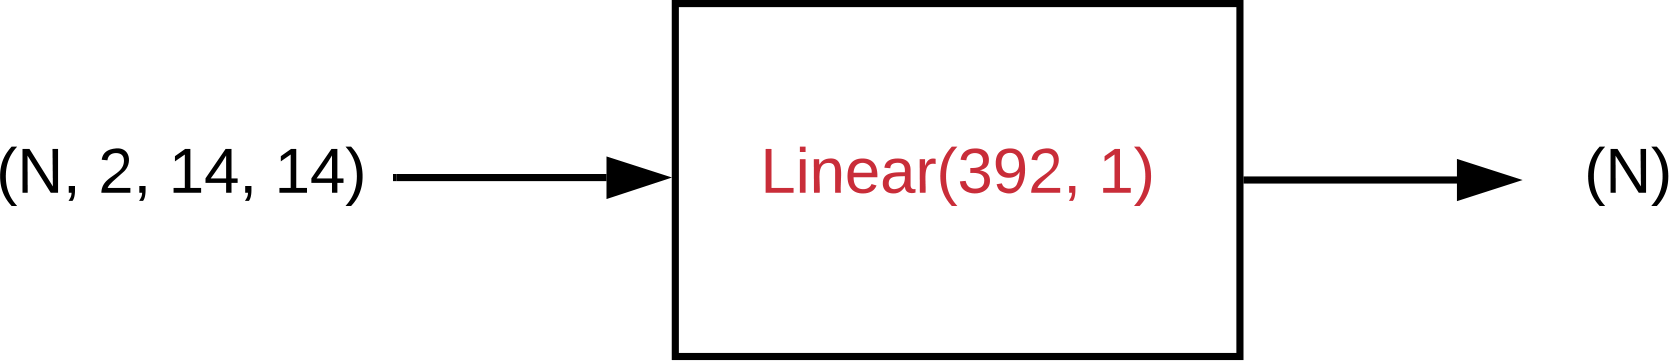
\includegraphics[width=0.35\textwidth]{linearregression.png}
    \caption{Linear Regression model}
    \label{fig:linearregression}
\end{figure}

\begin{figure}[!h]
    \centering
    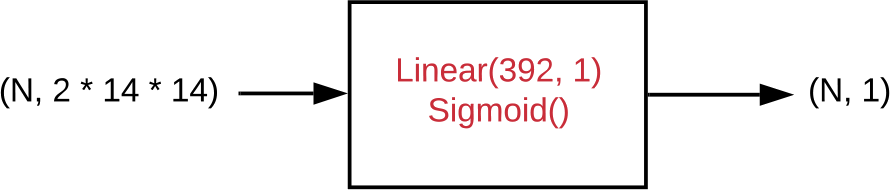
\includegraphics[width=0.35\textwidth]{logistic.png}
    \caption{Logistic Regression model}
    \label{fig:logisticregression}
\end{figure}

\section{Neural Network Models}
\label{sec:nnmodel}
We have implemented two models for neural network, the first one with 1 loss and the second one with 2 losses, as showed in Fig. \ref{fig:nn1} and Fig. \ref{fig:nn2}. Both models use the same feature extractors but they differs for the classifier(s). The first one has a boolean classifier that compares the two digits visible in the two images. The second model, it has also a digit classifier that returns the corresponding digit for both the handwritten images (class classification: we have used an hot encoding to give a target to each node).
For these two models the inputs are passed as 2D images. %TODO:sure? o é considerato come vettore?
Since the feature extractor processes both images together (it does not consider the two images independently), we can use a digit classifier with $20$ nodes as output ($10$ nodes for each images; i.e. from $0$ to $9$ as value of digit). We have noticed that NN with 2 losses seems to perform worst during the test then the model with 1 loss (see Table \ref{table:accuracy}). That seems to be in contrast with what we would expected; two losses could improve the accuracy if the model is more complex, otherwise it would affect negatively the accuracy (as in our case). Since we just have linear layers we could have improved the computation considering both the images independently. We have then decided to implement a convolutional neural network, since \textit{conv3d} allow to automatically process both the images independently.
\begin{figure}[!h]
    \centering
    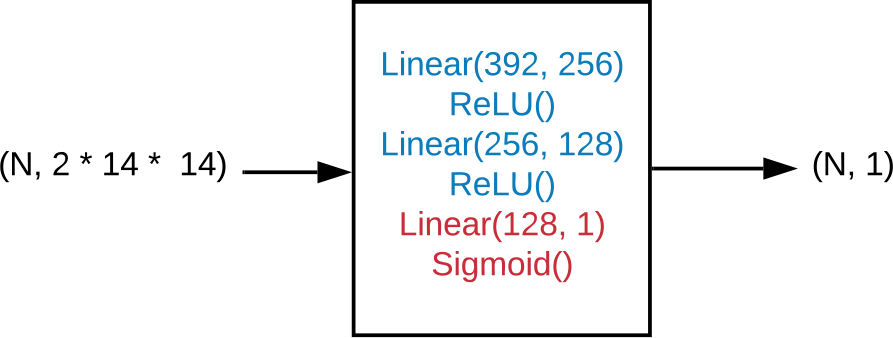
\includegraphics[width=0.35\textwidth]{nn1.png}
    \caption{Neural Network model (1 loss)}
    \label{fig:nn1}
\end{figure}

\begin{figure}[!h]
    \centering
    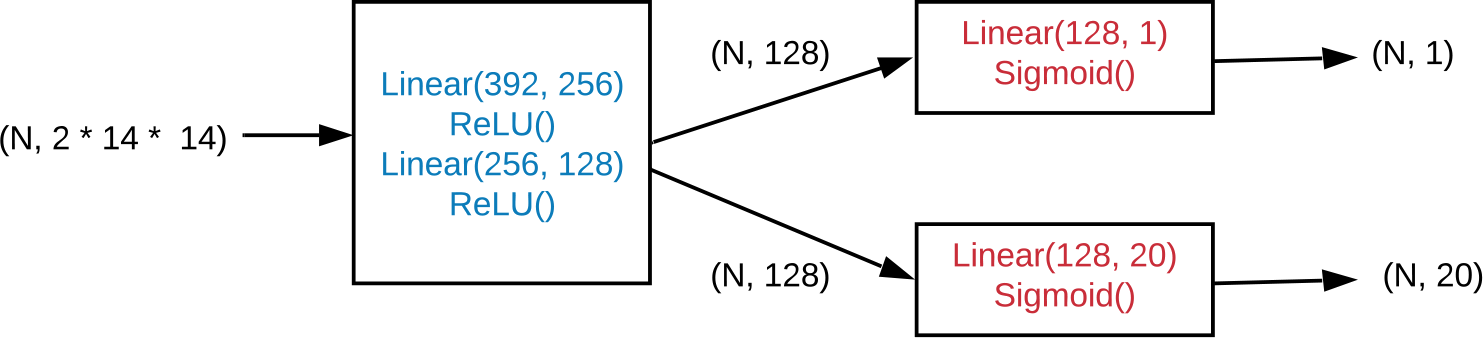
\includegraphics[width=0.5\textwidth]{nn2.png}
    \caption{Neural Network model (2 losses)}
    \label{fig:nn2}
\end{figure}


\section{Convolutional Neural Network Models}
\label{sec:cnnmodel}
Two models of convolutional neural networks were trained, both received an input of 3D images since we have decided to use a \textit{conv3d}. Conv3d are powerful cnn filter that are able to traverse the image in \textit{x}, \textit{y} and \textit{z} axes; that make possible to independently process both the two images. CNN are powerful since they use pixel locality, instead of flatting the input as done in previous model we consider the two 3D images. As done with the model of NN, in Sec. \ref{sec:nnmodel}, we have decided to compare two models one with one loss and the other one with two losses (see Fig. \ref{fig:cnn1} and Fig. \ref{fig:cnn2}). 
We have used the dropout to generalize better and then obtain a more robust model. CNN with 2 losses got the best accuracy with $84\%$  (see Table \ref{table:accuracy}).
\begin{figure}[!h]
    \centering
    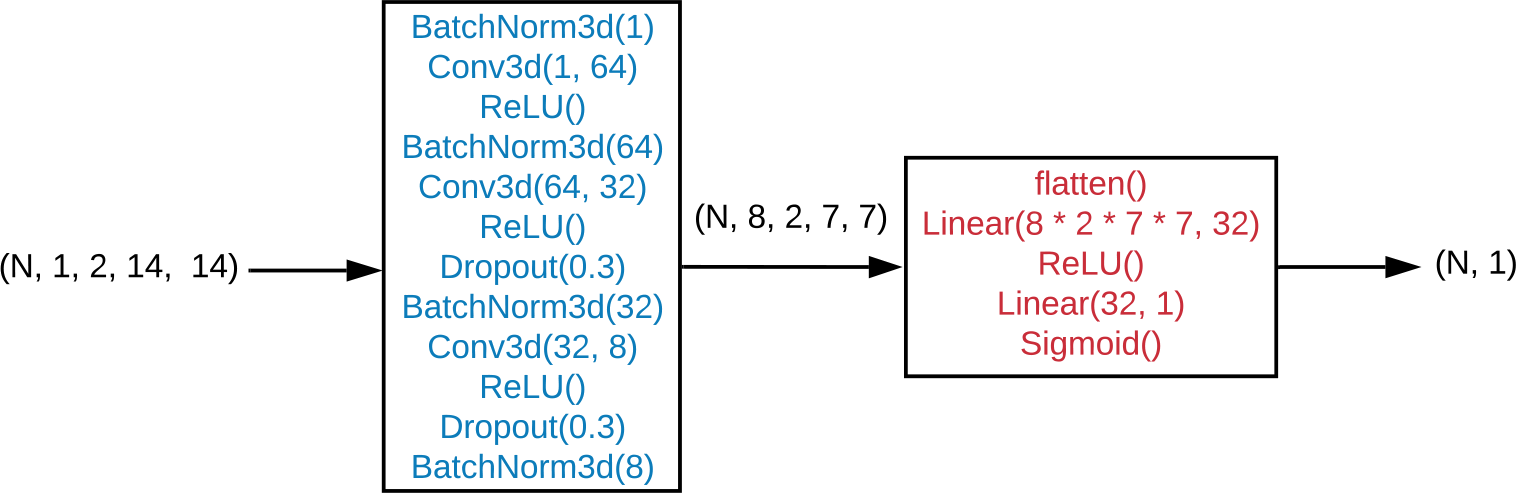
\includegraphics[width=0.5\textwidth]{cnn1.png}
    \caption{Convolutional Neural Network model (1 loss)}
    \label{fig:cnn1}
\end{figure}
\begin{figure}[!h]
    \centering
    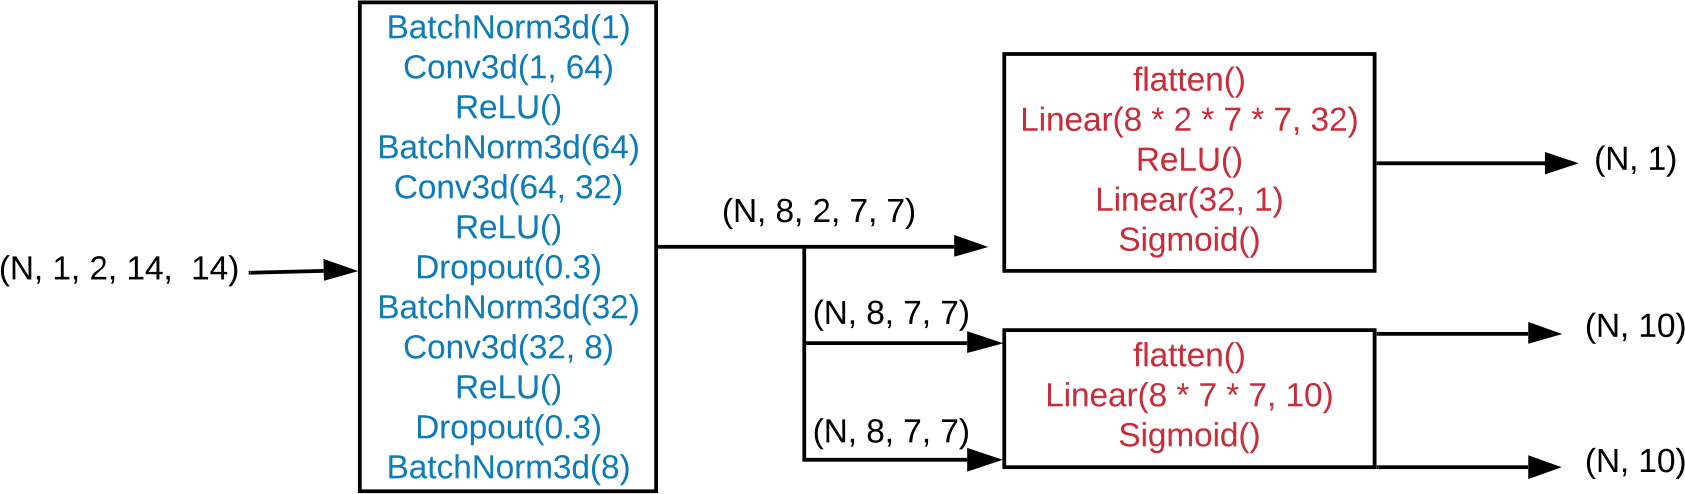
\includegraphics[width=0.5\textwidth]{cnn2.png}
    \caption{Convolutional Neural Network model (2 losses)}
    \label{fig:cnn2}
\end{figure}

\section{Comparison between 1 loss and 2 losses}
\label{sec:auxilaryloss}
We have decided to train the Neural Network and Convolutional Neural Network models also with an auxiliary loss. In addition of the loss obtained with the boolean classifier, we have added a new classifier that should detect the digit class of both images (the target is then an n-hot-encoding). Solving two tasks in parallel can help the model to extract a better representation of the data. The use of an auxiliary loss improved of $2\%$ the accuracy in CNN model.

\section{Comparison of models}
\label{sec:comparison}
Since linear models are really sensible to the weights setting 
we have decided to use a cross validation to compare the models (however, we did not implement our cross validation with \textit{pytorch}, we have used the library \textit{sklearn}).
Table \ref{table:params} summarizes all the number of parameters for each model. As expected neural networks require more parameters to got a good accuracy since they do not have weight sharing. Convolutional neural networks use weight sharing (a weight for all the pixels of the same filter) then it requires less parameters to got a good accuracy.

Plotboxs (see Fig. \ref{fig:train_acc_box}) show the accuracies for each models (using cross validation). We can notice that the accuracy vary a lot in simple models since they highly depend from weights initialization.

\begin{figure}[!h]
    \centering
    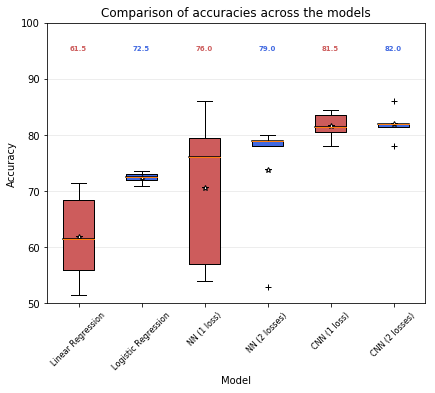
\includegraphics[width=0.5\textwidth]{boxplot.png}
    \caption{Plotbox that show the accuracy using cross validation. Star symbols represent the average values.}
    \label{fig:train_acc_box}
\end{figure}

\begin{table}
\centering
\caption{Table with number of parameters for each model.}
\label{table:params}
\begin{tabular}{|l|l|l|} 
\cline{3-3}
\multicolumn{1}{l}{} &                     & \textbf{Parameters}  \\ 
\cline{3-3}
\hline
                     & Linear Regression  & 393     \\ 
\cline{2-3}
               & Logistic Regression & 393     \\ 
\cline{2-3}
 \textbf{Models}   & NN (1 loss)~        & 133633  \\ 
\cline{2-3}
                     & NN (2 losses)~      &  136213  \\ 
\cline{2-3}
                     & CNN (1 loss)~       & 47803   \\ 
\cline{2-3}
                     & CNN (2 losses)     & 51733   \\
\hline
\end{tabular}
\end{table}

Table \ref{table:accuracy} shows the comparison between the accuracy obtained during the cross validation and the one in test. We can notice that test accuracy got better scores because we have used a bigger dataset to train. The dataset used in cross validation was $4/5$ of the total train set, instead the one used to test at the end was $5/5$ (all) of the dataset.
\begin{table}
\centering
\caption{Table accuracy (Cross validation: mean $\pm$ std).}
\label{table:accuracy}
\begin{tabular}{|l|l|l|l|} 
\cline{3-4}
\multicolumn{1}{l}{} &                     & \multicolumn{2}{c|}{\textbf{Accuracy}}  \\ 
\cline{3-4}
\multicolumn{1}{l}{} &                     & Cross validation & Test                 \\ 
\hline
                     & Linear Regression   & $61.8\pm7.467$    & $69.2$                 \\ 
\cline{2-4}
     & Logistic Regression & $72.4 \pm0.860$    & $73.8$                 \\ 
\cline{2-4}
\textbf{Models}    & NN (1 loss)~        & $70.5 \pm12.696$   & $80.5$                 \\ 
\cline{2-4}
                     & NN (2 losses)~      & $73.8 \pm10.419$   & $78.4$                 \\ 
\cline{2-4}
                     & CNN (1 loss)~       & $81.6 \pm2.289$    & $81.7$                 \\ 
\cline{2-4}
                     & CNN (2 losses)      & $81.9 \pm2.538$    & $83.7$                 \\
\hline
\end{tabular}
\end{table}

\section{Conclusion}
\label{sec:conclusion}
Convolutional Neural Network represents the best model with images recognition. In particular, the CNN with 2 losses seems to perform slightly better since it is able to extract better the data. We have seen that weight sharing (CNN) improves the accuracy and the robustness of the model, the use of an auxiliary loss in this context improves the results obtained.

As future improvement we would like to implement the cross validation using the \textit{pytorch} library.
% %%%%%%%%%%%%%%%%%%%%%




% Now we need a bibliography:
\begin{thebibliography}{999}

	%Each item starts with a \bibitem{reference} command and the details thereafter.
	\bibitem{reference0}
    	optim.Adam vs optim.SGD. Let’s dive in.
    	\url{https://medium.com/@Biboswan98/optim-adam-vs-optim-sgd-lets-dive-in-8dbf1890fbdc}
	
% 	\bibitem{reference1}
% 	    Neural networks and deep learning, Michael Nielsen.
	    
%     \bibitem{reference2}
%     Notes of course Deep Learning (EE-559), Prof. François Fleuret.

\end{thebibliography}

% Your document ends here!
\end{document}

% \begin{table}
% \centering
% \caption{Table with number of parameters for each model.}
% \label{table:params}
% \begin{tabular}{|l|l|l|l|l|} 
% \cline{3-5}
% \multicolumn{1}{l}{} &                     & \multicolumn{3}{c|}{\textbf{Parameters}}          \\ 
% \cline{3-5}
% \multicolumn{1}{l}{} &                     & Feature extractor & Classifier & Total   \\ 
% \hline
%                      & Linear Regression   & -                 & 393        & 393     \\ 
% \cline{2-5}
%               & Logistic Regression & -                 & 393        & 393     \\ 
% \cline{2-5}
%  \textbf{Models}   & NN (1 loss)~        & 133504            & 129        & 133633  \\ 
% \cline{2-5}
%                      & NN (2 losses)~      & 133504            & 129        & 136213  \\ 
% \cline{2-5}
%                      & CNN (1 loss)~       & 22650             & 25153      & 47803   \\ 
% \cline{2-5}
%                      & CNN (2 losses)      & 22650             & 25153      & 49773   \\
% \hline
% \end{tabular}
% \end{table}